\section{Application: finding optimal DR-plans and realizations for cross-linking microfibrils }
\label{sec:pinnedline}

The canonical DR-plan of Section \ref{sec:DRP} can also be applied to analyze and solve
the structure of  cross-linking collagen and cellulose microfibrils
in animal and plant cell walls, and actin filaments in the cytoskeleton
by modeling these structures as \dfn{pinned line-incidence systems}.


\dfn{Collagen} is an important protein material in biological tissues with highly elastic mechanical property \cite{buehler2008nanomechanics}.
\dfn{Cellulose} is the most important constituent of the cell wall of plants (see Figure~\ref{fig:cellulose}) \cite{fall2013physical,smith1971plant}.
Both of these substances consist of a large number \dfn{microfibrils},
%fibril itself straight?
%Each fibril is attached to some fixed larger organelle/membrane at one spot (typically on the boundary).
%It is additionally
each of which is cross-linked at 2 places with usually 3 other fibrils,
where the \dfn{cross-linking} is like an incidence constraint that the
crosslinked fibrils can slide against each other while remaining incident (see
Figure~\ref{fig:crosslink}).

%Collagen
%
%layers of microfibril with cross-linking???
%
%
%- different cross-linking densities
%larger cross-link densities lead to larger yield strains, larger yield stresses as well as larger fracture stresses.
%the maximum fracture stress of the collagen fibril does not increase with increasing cross-link densities (2 links per molecule)
%
%
%Plant cell wall, cellulose
%
%Non-charged cellulose is considered to form a random mesh, the rigidity of which would depend on the number of interfibriller cross links, i.e. H bonds.
%new microfibrils were laid down on top of the existing ones, forming a new layer.


\begin{figure}
\centering

\begin{subfigure}{.49\linewidth}
  \centering
  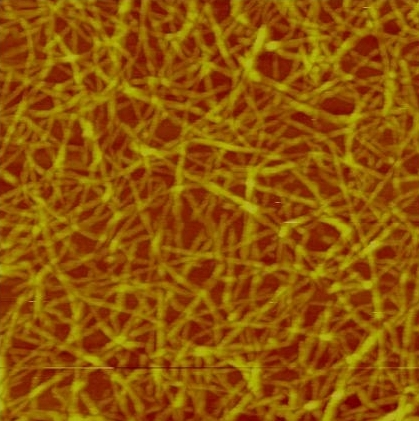
\includegraphics[width=.8\linewidth]{img/AFM_Innventia_nanocellulose}
  \caption{}
  \label{fig:cellulose}
\end{subfigure}
\begin{subfigure}{.49\linewidth}
  \centering
  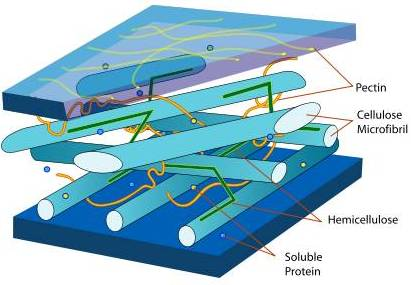
\includegraphics[width=\linewidth]{img/crosslink}
  \caption{}
  \label{fig:crosslink}
\end{subfigure}%
\caption{(a) Microfibrils of carboxymethylated nanocellulose adsorbed on a silica surface \cite{wikimediacommons2010afm}. (b) Cross-linking of cellulose microfibrils \cite{wikimediacommons2007plant}.}
\end{figure}






\subsection{Modeling the fibrils as a pinned line-incidence system}



The cross-linking microfibrils can be modeled as a pinned line-
incidence constraint system in $\mathbb{R}^2$, where incidence
constraints are used instead of distance constraints.

A \dfn{pinned line-incidence system} $(G,\delta)$ is a graph $G=(V,E)$
together with parameters $\delta$ specifying $|E|$ \textbf{pins} with
fixed positions in $\mathbb{R}^2$, such that each edge is constrained
to lie on a line passing through the corresponding pin, i.e.\ $\delta:
E \rightarrow \mathbb{R}^2$.
%
% $G=(V,E, w_V, w_E)$
%%is a \textbf{2-dimensional pinned line-incidence graph},
% has weight functions $w_V(v) = 2, w_E(e) = 1$ for all $v \in V, e \in E$.
%Additionally, there is  a  set $X$ of $|E|$ \textbf{pins} with fixed positions in $\mathbb{R}^2$,
%such that  %every edge $e \in E$ corresponds to a pin $x \in X$ where
%for each edge $e \in E$, there is a uniquely corresponding pin $x \in X$,
%such that $e$ is constrained to lie on a line passing through $x$.
%%There exists a set $X$ of $|E|$ pins fixed in $\mathbb{R}^2$, such that each edge $e_i$
%
A pinned line-incidence graph $G$ is rigid if $|E| = 2|V|$ and $|E'| \le 2|V'|$ for every induced subgraph $(V',E')$ \cite{sitharam2014incidence}. Note that no trivial motion exists since the pins have fixed positions on the plane.
Euclidean transformations are not factored out.
In particular, both a single vertex and a single edge are underconstrained graphs.




In the case of microfibril cross-linking, each fibril is
attached to some fixed larger organelle/membrane at one spot.
Consequently, each fibril can be modeled as an edge of the graph,
with the attachment being the corresponding pin.
The two cross-linkings on the fibril are modeled as the two vertices in $V$ defining the edge.



Figure~\ref{fig:pinned_line} shows an example of a pinned line-incidence graph,
where the grey ovals denote pins representing attachments of fibrils,
and the vertices $a_1,a_2,\ldots, c_3$ represent cross-linkings.
% and the black dots stand for vertices/cross-linkings.
%There are  and 10 vertices/cross-linkings in the graph.
The graph is isostatic, with 12 vertices and 24 edges/pins.

\begin{figure}
  \centering
   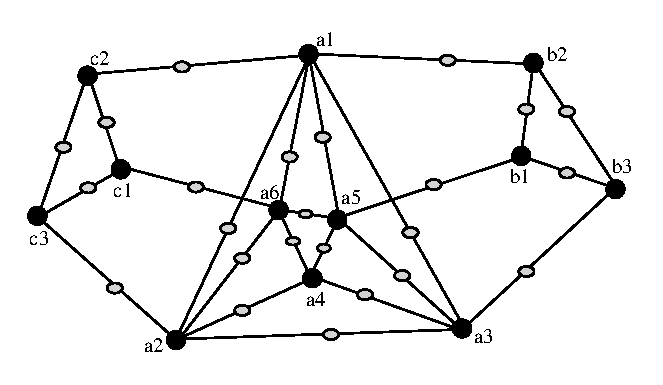
\includegraphics[width=.7\linewidth]{img/pinned}
\caption{ An isostatic pinned line-incidence graph.}
\label{fig:pinned_line}
\end{figure}


\subsection{Optimal DR-plan for pinned line-incidence systems}

%Recall the definitions in Section~\ref{priliminary}.

In this section, we will adapt the results in Section~\ref{sec:DRP}
to give the canonical DR-plan for pinned line-incidence graphs.
First, we note that %unlike bar-joint graphs,
\vemph{an isostatic pinned line-incidence graph can be disconnected},
being the disjoint union of two or more isostatic subgraphs.
This is because the pins have fixed positions on the plane.
%
%the following difference of pinned line-incidence graphs from the bar-joint graphs.
%
%For pinned line-incidence graphs,
%since the pins have fixed positions on the plane,
%{\em a wellconstrained vertex-maximal proper subgraph can be disconnected},
%being the disjoint union of two or more wellconstrained subgraphs.
%
%\begin{itemize}
%
%\item For pinned line-incidence graphs,
%since the pins have fixed positions on the plane,
%no trivial motion exists, therefore {\em no trivial overconstrained graphs exist} (the smallest overconstrained graph has $6$ vertices).\\
%In particular, note that both a single vertex and a single edge are underconstrained graphs.
%
%\item
%For pinned line-incidence graphs,
%since the pins have fixed positions on the plane,
%{\em a wellconstrained vertex-maximal proper subgraph can be disconnected},
%being the disjoint union of two or more wellconstrained subgraphs. \\
%%Without loss of generality,
%%we slightly modify the requirement of DR-plan for pinned line-incidence graphs
%%such that only connected subgraphs can be considered as a node of the DR-plan.
%
%\end{itemize}
%
We define a \dfn{trivial} graph to be a single vertex and make the following modification to the definition of
the canonical DR-plan:

%\begin{itemize}
%\item For any $C$, its $N$ children, $C_1, \ldots, C_N$, are {\em edges} or {\em connected} wellconstrained vertex-maximal proper subgraphs of that node $C$.
%\item A node containing a single edge is a leaf.
%%\item
%%\todo{We just define the %trivial graph/
%%DR-plan leaves for 2-dimensional pinned line-incidence graphs to be single vertices...  }
%%\item \todo{A single edge can be a node of the DR-plan}
%%\item only connected subgraphs can be considered as a node of the DR-plan.
%\end{itemize}

\begin{definition}
The \dfn{DR-plan} of a  pinned line-incidence graph $G$ is one in which
(1) each child node of a non-leaf node $C$ is either a \dfn{connected} rigid vertex-induced subgraph of $C$,
or an edge not contained in any  proper rigid subgraph of $C$, and (2) a leaf node is a single edge.
% Definition~\ref{def:drp} with  modified rules number 2 and 4:
%    The \textbf{decomposition-recombination (DR-) plan} of  a 2-dimensional pinned line-incidence graph $G$, $DRP(G)$, is  a tree that has the following properties:
%    \begin{enumerate}
%        %\item The root of the tree `contains' $G$.
%        \item[2] For any non-leaf node $C$, each of its children, $C_1,\ldots,C_N$, is either an edge not contained in any wellconstrained proper subgraph of $C$, or a {\em connected} wellconstrained vertex-maximal proper subgraph of  $C$.
%        %\item The vertex set of $\bigcup_{i=1}^N{C_i}$ is the vertex set of $C$.
%        \item[4] A node containing a single edge is a leaf.
%    \end{enumerate}

The \dfn{canonical DR-plan} of $G$  is one in which
the  children containing rigid subgraphs are connected isostatic vertex-maximal subgraphs of the parent.
\end{definition}


Theorem~\ref{theorem:main}
holds for  pinned line-incidence graphs with the above modified definition.
The proof is similar to the original proof (in the Appendix) using the same set of lemmas and
%
%\begin{corollary}\label{cor:pinned}
%Given a isostatic pinned line-incidence graph, for node $C$ in $OptimalDRP(G)$ and the children of $C$ in $CompleteDRP(C)$ labeled as $C_1,\ldots,C_N$
%\begin{enumerate}
%    \item if $C_i \cap C_j$ is trivial then all $C_1,\ldots,C_N$ are children of $C$ in $OptimalDRP(G)$.
%    \item if $C_i \cap C_j$ is isostatic then any two out of $C_1,\ldots,C_N$ will be the only children of $C$ in $OptimalDRP(G)$.
%\end{enumerate}
%\end{corollary}
%
the following modified version of Observation~\ref{lemma:union_intersection},
% observation, which
%serves a similar function to Observation~\ref{lemma:union_intersection} in Section~\ref{sec:DRP}
%Using similar counting-based argument, %  to Lemma~\ref{t-l1}--\ref{iuc-l1} in Section~\ref{sec:union_intersection},
which  can be proved using a simple counting based argument.


\begin{observation}\label{lem:pinned_union_intersection}
Let $F_i$ and $F_j$ to be subgraphs of the same isostatic graph $F$,
where each of them can be either a single edge or a connected isostatic subgraph.
There are only two possible cases:
(1) At least one of $F_i$, $F_j$ is an edge, if and only if $F_i \cup F_j$ is underconstrained, if and only if $F_i \cap F_j$ is trivial; and (2) both $F_i$ and $F_j$ are isostatic, if and only if $F_i \cup F_j$ is isostatic, if and only if $F_i \cap F_j$ is isostatic.
%The following table summarizes all bijections:
%\setlength{\tabcolsep}{3pt}
%{\small
%\begin{center}
%\begin{tabular}{|p{2.8cm}|c|p{2.3cm}|}
%\hline
%\textbf{Property of $F_i,F_j$} & \textbf{$F_i\cup F_j$} & \centering \textbf{$F_i\cap F_j$}  \tabularnewline \hline
% \centering--- &  \sout{overconstrained}          &  \centering --- \tabularnewline \hline
%at least one of $F_i,F_j$ is an edge & underconstrained       &  \centering a vertex (underconstrained)  \tabularnewline \hline
%both $F_i$ and $F_j$ are wellconstrained & wellconstrained        &  \centering wellconstrained  \tabularnewline \hline
% \centering --- & ---                     &  \centering \sout{underconstrained} \tabularnewline \hline
%\end{tabular}
%\end{center}
%}
%\setlength{\tabcolsep}{6pt}
\end{observation}

Given Lemma~\ref{lem:pinned_union_intersection}, % and the modified definition of DR-plan,
Lemma~\ref{lemma:wc_intersection_is_C} and \ref{lemma:uc_intersection_makes_all_uc} straightforwardly extend to  pinned line-incidence graphs. The proof of Lemma~\ref{lemma:wc_intersection_makes_all_wc} for pinned
line-incidence graphs is given in Appendix~\ref{sec:appendix_pinned}.
%The following lemma serves as Lemma~ for pinned line-incidence and can be proved similarly.
%\begin{lemma}
%\label{lem:vertex_intersection}
%If $C_i\cap C_j$ is a single vertex, then $\forall k: C_i\cap C_k$ is a single vertex.
%\end{lemma}
%Given Lemma~\ref{lemma:wc_intersection_makes_all_wc} and Lemma~\ref{lemma:uc_intersection_makes_all_uc},
Thus it is straightforward to adapt the proof of Theorem~\ref{theorem:main}
to  pinned line-incidence graphs.
%thus proving Corollary~\ref{cor:pinned}.
%
Consequently, we can efficiently find the optimal DR-plan for  pinned line-incidence graphs using basically the same algorithm as for  bar-joint graphs.

\noindent
\note The recombination problem for  pinned line-incidence systems is trivial.
Since the pins are given fixed positions in the plane,
the solutions of a isostatic sub-system will automatically be consistent with solutions of the remaining of the system.


